\documentclass[a4paper,10pt,titlepage]{article}
\usepackage{color}
\usepackage{wrapfig}
\usepackage[dvipdfm]{geometry}
\usepackage{amsmath}
\usepackage{amsfonts}
\usepackage[utf8]{inputenc}
\usepackage{amssymb}
\usepackage{graphicx}
\usepackage{fancyhdr}
\usepackage{svnkw}
\usepackage{tabularx}
\usepackage{ngerman}
\pagestyle{fancy}
\evensidemargin0mm
\oddsidemargin0mm
\setlength{\listparindent}{0pt}
\setlength{\parskip}{0pt}
\voffset-10mm
\topmargin0mm
\headsep10mm
\headheight20mm
%\svnid{$Id: pflichtenheft.tex 25 2009-10-15 18:17:25Z heins4 $}
\lhead{
\includegraphics{bfh_logo.png}\newline}
\rhead{Stefan Heinemann (heins4)\\Christoph Isch (ischc2)}
\lfoot{\today}

\title{Documentation}
\author{heins4: Stefan Heinemann\\ischc2: Christoph Isch}
\begin{document}

\begin{titlepage}
{\huge Project Specifications}\\
\textbf{heins4: Stefan Heinemann}\\
\textbf{ischc2: Christoph Isch}\\
%\textbf{reutm1: Michel Reuteler}\newline\newline\newline\newline\newline\newline\newline\newline
%\emph{Last changed: \svnkw{LastChangedAt}}\newline
%\emph{Revision: \svnkw{LastChangedRevision}}\newline\newline\newline\newline
\newline\newline\newline\newline\newline
\newline\newline\newline\newline\newline\newline\newline\newline\newline
\newline\newline\newline\newline\newline\newline\newline\newline

\includegraphics[width=40mm]{bfh_logo.png}\newline

\emph{Modul: Projektarbeit 2 (7302r)}\newline
\emph{Professor: Prof. Dr. Jürgen Eckerle}

\end{titlepage}
%Der Begriff \emph{Verkehrsstau} (kurz Stau) bezeichnet einen stark stockenden oder zum Stillstand gekommenen Verkehrsfluss auf einer Straße. Als einer der Gründe dafür gilt eine zu hohe Anzahl von Fahrzeugen pro Zeiteinheit und Streckenlänge. Die Ursachen für einen Verkehrsstau sind damit allein jedoch nicht erklärbar.\newline
%Verkehrsexperten legen Wert darauf, zwischen \glqq Stau\grqq\space und \glqq stockendem Verkehr\grqq\space zu unterscheiden. In der Schweiz beispielsweise wird \glqq fachlich\grqq\space von einem Stau gesprochen, wenn der Verkehr mindestens für eine Minute mit weniger als 10 km/h fließt. Liegt die Geschwindigkeit im Bereich zwischen 10 und 30 km/h, spricht man von stockendem Verkehr.
%\newline\newline\newline
%\begin{center}
% \includegraphics[width=8cm]{./traffic-jam.jpg}
 % traffic-jam.jpg: 500x333 pixel, 72dpi, 17.64x11.75 cm, bb=0 0 500 333
%\end{center}

%\newpage

\tableofcontents


\newpage

\section{Disposition}

\subsection{Problem description}
%We have to implement an event driven traffic simulation.
Our task is to implement an event driven traffic simulation based upon a driver model, an environmental model and a vehicle model.
%Im Rahmen des Projektfachs der Berner Fachhochschule ist unsere Aufgabe, eine
%Event-Gesteuerten Verkehrssimulation basierend auf einem Fahrermodell, Strassenmodell
%und Fahrzeugmodell zu implementieren.

%\subsection{Target}
We have to provide models and simulate street traffic. 
The simulation is divided in three models:

%In unserem Projekt geht es um Modellierung und Simulation von Strassenverkehr.
%Die Simulation ist in drei Modelle aufgeteilt

\begin{enumerate}
 \item Environmental Model%Umgebungsmodell
 \item Driver Model%Fahrermodell
 \item Vehicle Model%Fahrzeugmodell
\end{enumerate}
The environmental and vehicle models have been mostly implemented already in our work in module 7301r. This project is based on that work.
%Das Umgebungsmodell und das Fahrzeugmodell wurde in grossen Zügen bereits im Modul 7301r erstellt. Dieses Projekt baut auf unserer damaligen Arbeit auf.

\begin{center}
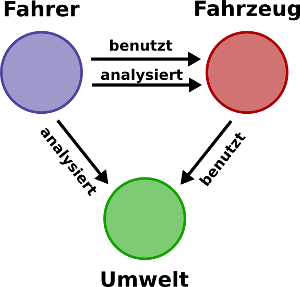
\includegraphics[width=5.5cm]{skizze.png}
\end{center}

\subsection{Objectives}
\subsubsection{Driver model}
 Create a parameterised driver model to be able to implement different 
 driver characters. These characters will be able to drive around autonomously 
 and make decisions based on the circumstances that they see and will be 
 influenced by parameters such as ``riskyness'' and temperament or drug intake.
 We are trying to achieve a high complexity in this field.



%Realisierung eines parametrisierbaren Fahrermodells (um den %
%unterschiedlichen Fahrertypen gerecht zu werden) bestehend aus einer %
%Vielzahl von Basisfahrmustern, hohe komplexität angestrebt}

\subsubsection{Display}

Display the current state of the traffic situation. %Graphische Darstellung der Verkehrssituation
\newpage

\subsection{Optional Objectives}
\begin{enumerate}
 \item Changing the behaviour of the drivers by showing them road signs. %Weitere Standardsituationen wie kompliziertere Kreuzungen, Kreisel oder Ampeln
 \item Obstruction of the view by buildings etc. %Physikalisch komplexere Modelle (3D, Reibung, Kurvenfahrt)
\end{enumerate}
%\begin{center}
%  \includegraphics[width=7cm,keepaspectratio=true]{./kreisel.jpg}
  % kreisel.jpg: 617x606 pixel, 72dpi, 21.77x21.38 cm, bb=
  %\caption{Beispiel eines Kreisels}
%\end{center}

\subsection{Learning Goals}
Creation of an event driven simulation, applying basic principles of AI in the driver model.
%Aufbau einer Event-Gesteuerten Simulation. Verständnis der zugrundeliegenden
%Algorithmen.


\section{Organisation}

\subsection{Used Software}
\begin{tabular}{ll}
Programming Language & Java 6 \\
& \\
IDE & Eclipse \\
& \\
Documentation & \LaTeX \\
& \\
Version control & git \\
\end{tabular}

\subsection{Version control}
The version control is done with the free Tool Git\footnote[1]{http://git-scm.com}.
An online repository is hosted on github: \newline
http://github.com/schtibe/Projektarbeit-2-7302

%Die Versionskontrolle erfolgt über das freie Tool Subversion\footnote[1]{http://subversion.tigris.org/}.\newline 
%Das Subversion Repository befindet sich unter \newline
%https://svn.bfh.ch/repos/projects/projektarbeit7301r.\newline\newline

\subsection{Involved Persons}

\begin{tabularx}{\textwidth}{XXX}
 Jürgen Eckerle & Professor & juergen.eckerle@bfh.ch \\
 Stefan Heinemann & Developer & heins4@bfh.ch \\
 Christoph Isch & Developer & ischc2@bfh.ch \\
\end{tabularx}

\subsection{Dates}

Start: 20.09.2010 \\
End: End of fall term 10/11

\section{System Requirements}

\subsection{Hardware}
\begin{enumerate}
 \item Intel Core 2 Duo
 \item 2 GB RAM
 \item GFX Card with 128 MB RAM
\end{enumerate}

Depending on the amount of simulated vehicles, the minimal requirements may not be sufficient.

%Je nach Grösse der Simulation kann die Anforderung an die Hardware
%stark varieren.

\subsection{Software}
\begin{enumerate}
 \item Java Virtual Machine
\end{enumerate}


\section{Results}

The final results will be delivered in a zipped file.
%Das Endergebnis wird in einem ZIP-File abgeliefert.

\subsection{Application}
\begin{enumerate}
 \item Executable jar-file%Ausführbares Jar-File
 \item Sourcecode
\end{enumerate}

\subsection{Documentation}
\begin{enumerate}
 \item Project Specifications
 \item Javadoc
 \item Final Report
 \item Implementation
 \item Set up instructions
\end{enumerate}

All documents and all in-line documentation in code will be written in English.

%Alle Dokumente werden in deutscher Sprache verfasst. Die Dokumentation
%innerhalb des Sourcecodes erfolgt in Englischer Sprache.\footnote[2]{blah} \newline\newline

\newpage
\begin{tabularx}{\textwidth}{XXX}
\textbf{Version} & \textbf{Date} & \textbf{Comment}\\
1 & 05.10.10 & \\
%2 & 6.09.09 & \\
%3 & 7.09.09 & \\
%4 & 12.09.09 & \\
\end{tabularx}


\end{document}
